\chapter*{Apéndice A. Funciones para Mathematica}
\section*{Aproximación de raíces}


\section*{Sistemas de ecuaciones lineales}

\section*{Interpolación polinómica}
\noindent \textbf{Diferenciadiv[f,$\mathbf{\{x_o,\ldots,x_n\}}$]:} calcula $f[x_o,\ldots,x_n]$.
        \begin{figure}[h]
            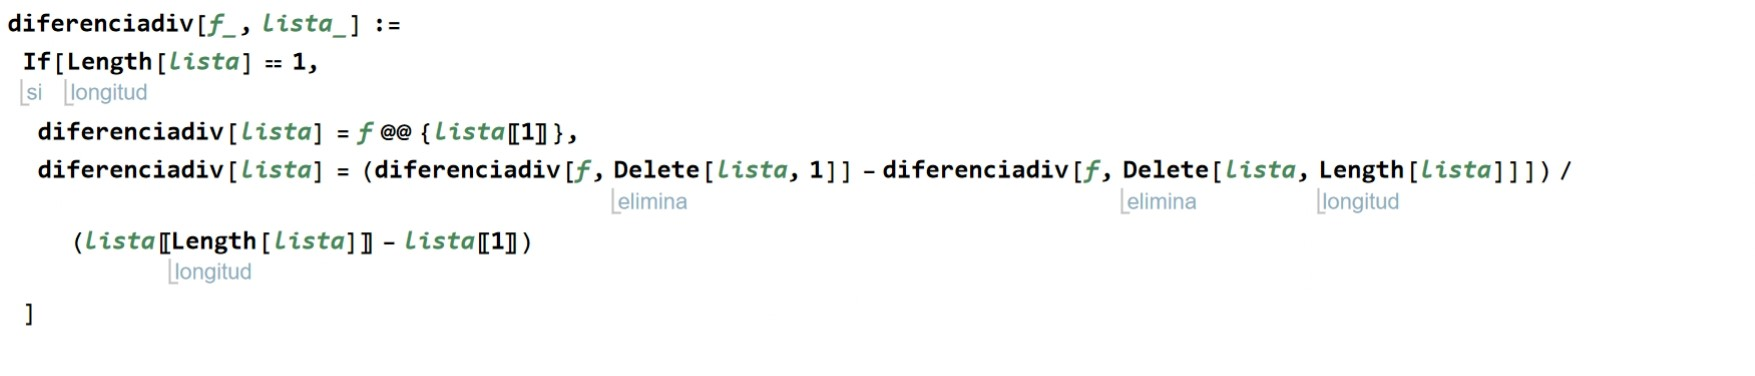
\includegraphics[scale=0.60]{diferencias_divididas.jpg}
        \end{figure}
        
        \noindent \textbf{tabladifdiv[f,$\mathbf{\{x_o,\ldots,x_n\}}$]}: la salida es una tabla con las diferencias divididas $f[x_i,\ldots,x_{j+i}]$ con $i\in\{0,\ldots,n\}$ y $j+i\leq n$
                \begin{figure}[h]
            \centering
            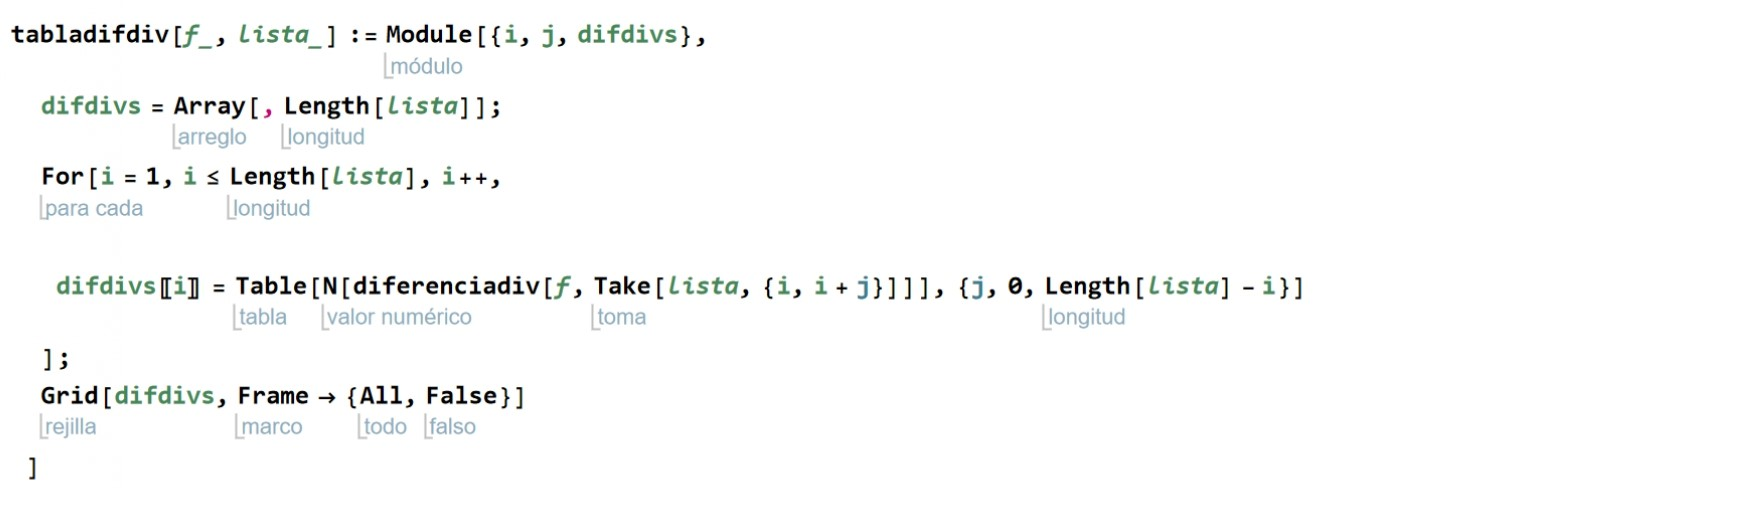
\includegraphics[scale=0.6]{yepa_page-0001.jpg}
        \end{figure}
        
        \noindent \textbf{chebyshev[n]}: calcula el polinomio $T_n(x)$.
          \begin{figure}[h]
            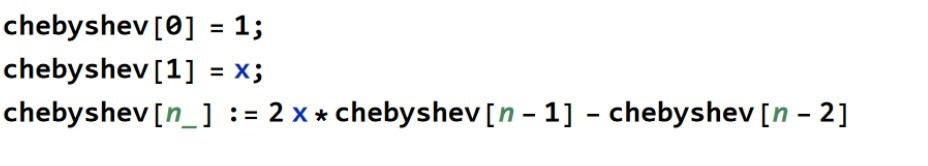
\includegraphics[scale=0.60]{yepa_page-0001 (1).jpg}
        \end{figure}
        
       \noindent \textbf{Plotchebyshev[n]:} si $n\geq 0$ la salida es un gráfico del polinomio $T_n(x)$ y si \newline $n=\{n_1,n_2\}$ la salida es un gráfico de los polinomios $T_{n_1}$ hasta el $T_{n_2}$ .
        
        \begin{figure}[h]  
            \centering
            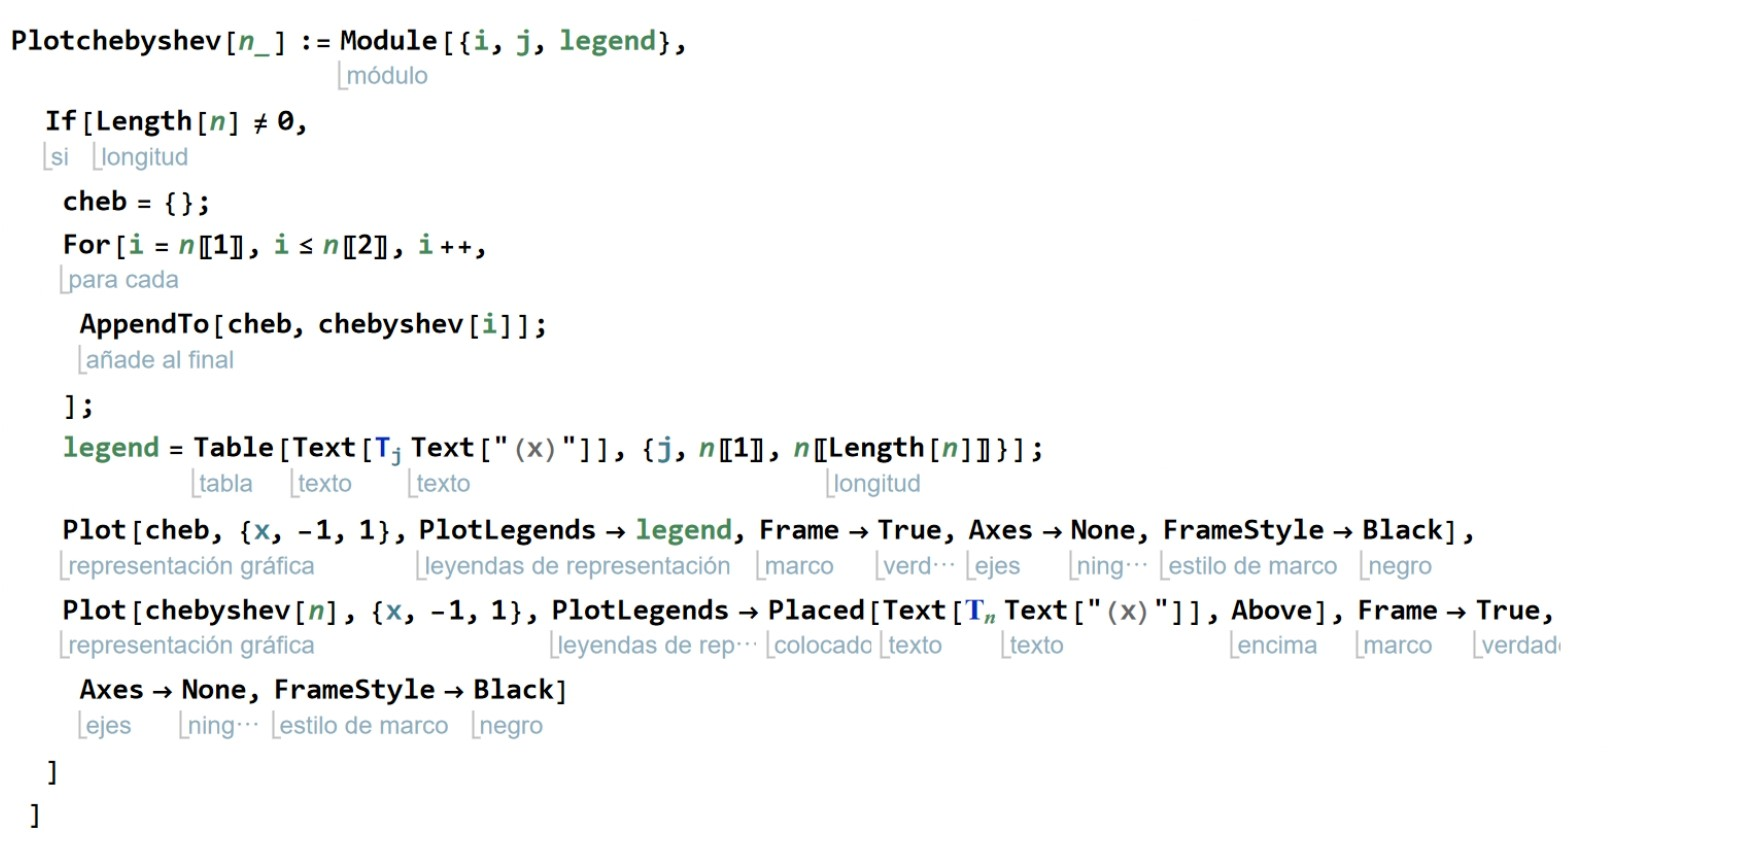
\includegraphics[scale=0.6]{yepa_page-0001 (2).jpg}
        \end{figure}
              \newpage
        \noindent \textbf{Nodoschebyshev[n,\{a,b\}]:} calcula los $n$ primeros nodos de Chebyshev del intervalo $(a,b)$.
        \begin{figure}[h]
            \centering
            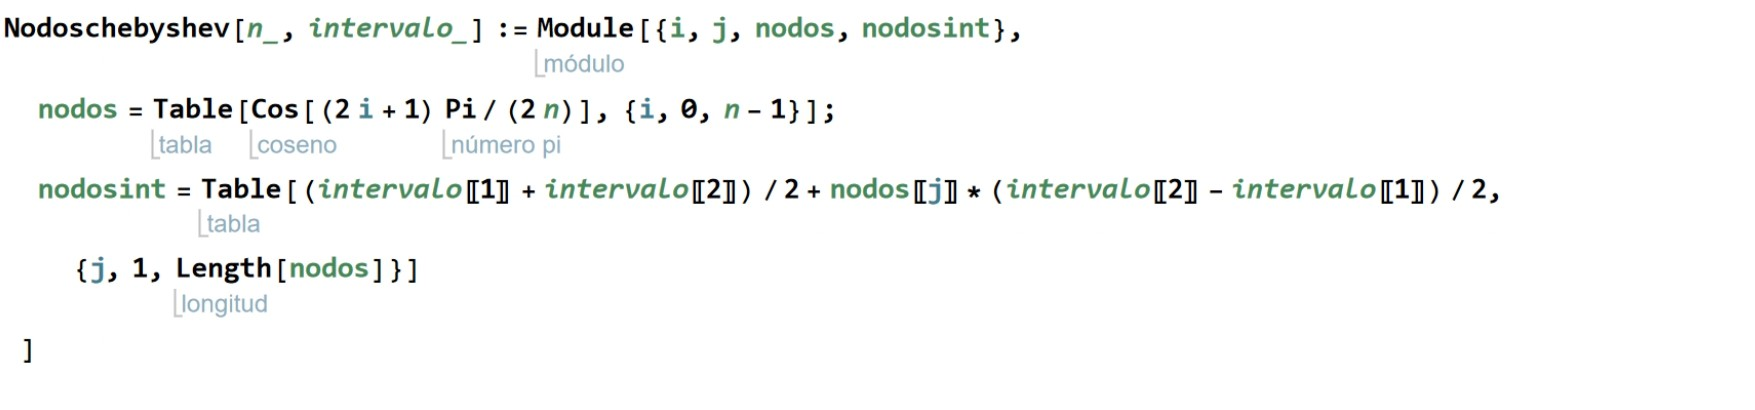
\includegraphics[scale=0.6]{yepa_page-0001 (3).jpg}
        \end{figure}
  
        \noindent \textbf{ChebyshevInt[f,n,\{a,b\}]:} hace un gráfico de la función $f$ junto con el polinomio de interpolación de dicha función en los $n$ primeros nodos de Chebyshev del intervalo $(a,b)$.
        
        \begin{figure}[h]
            \centering
            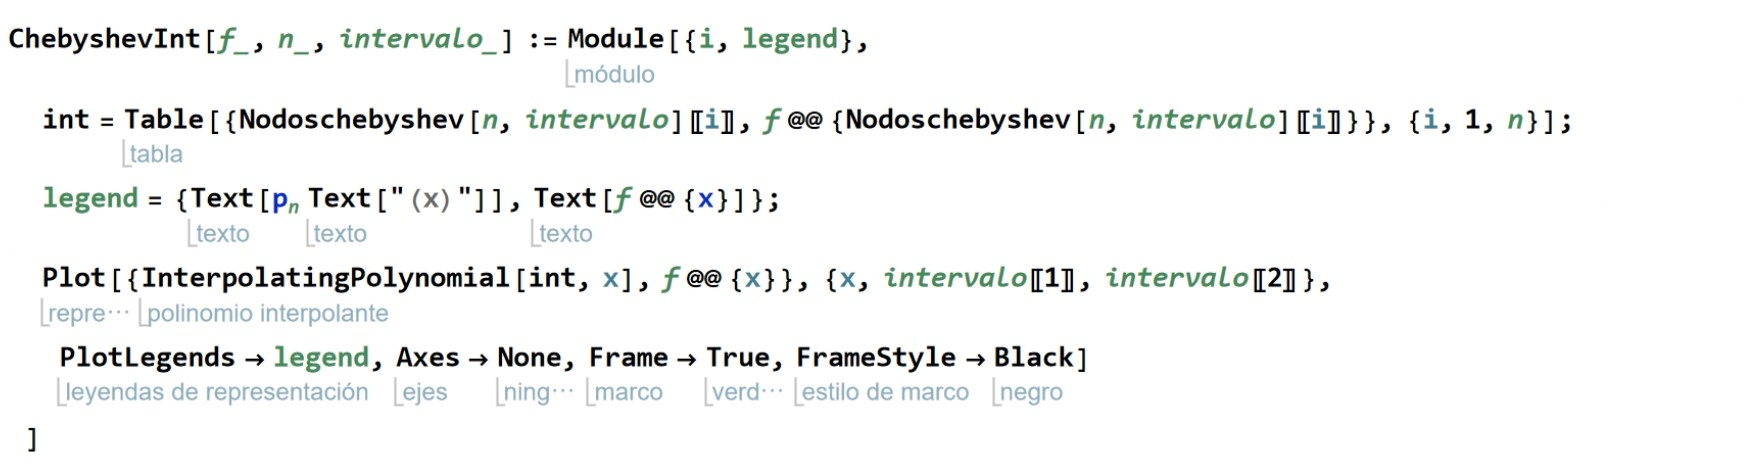
\includegraphics[scale=0.55]{yepa_page-0001 (4).jpg}
        \end{figure}